\documentclass[a4paper]{article}

%use the english line for english reports
%usepackage[english]{babel}
\usepackage[portuguese]{babel}
\usepackage[utf8]{inputenc}
\usepackage{indentfirst}
\usepackage{graphicx}
\usepackage{verbatim}
\usepackage{listings}
\usepackage{booktabs}

\begin{document}

\setlength{\textwidth}{16cm}
\setlength{\textheight}{22cm}

\title{\Huge\textbf{Gestão de Elevadores}\linebreak\linebreak\linebreak
\Large\textbf{Relatório Final}\linebreak\linebreak
\linebreak\linebreak

\includegraphics[scale=0.1]{feup-logo.png}\linebreak\linebreak
\linebreak\linebreak
\Large{Mestrado Integrado em Engenharia Informática e Computação} \linebreak\linebreak
\Large{Agentes e Inteligência Artificial Distribuída}\linebreak
\Large{4º Ano 1º Semestre}\linebreak\linebreak
}

\author{\textbf{Grupo T01\_3:}\\ Luís  Barbosa - 201405729 - up201405729@fe.up.pt\\ Paulo Santos - 201403745 - up201403745@fe.up.pt \\ Sérgio Almeida  - 201403074 - up201403074@fe.up.pt \\\linebreak\linebreak \\
 \\ Faculdade de Engenharia da Universidade do Porto \\ Rua Roberto Frias, s/n, 4200-465 Porto, Portugal \linebreak\linebreak\linebreak
\linebreak\linebreak\vspace{1cm}}
\date{10 de dezembro de 2017}
\maketitle
\thispagestyle{empty}

%************************************************************************************************
%************************************************************************************************

\newpage

\tableofcontents

%************************************************************************************************
%************************************************************************************************

%*************************************************************************************************
%************************************************************************************************

\newpage

%%%%%%%%%%%%%%%%%%%%%%%%%%
\section{Objetivo}

\subsection{Descrição do cenário} 

O cenário do presente trabalho consiste num edifício de vários andares com diversos elevadores. Cada elevador possui uma carga máxima, que corresponde ao número máximo de pessoas que pode transportar.

Os elevadores comunicam entre si informação relevante. Quando há um novo pedido numa determinada zona do edifício, este deve ser alocado a um dos elevadores existentes naquela zona. Os elevadores possuem uma lista de pisos em que têm que parar, podendo a mesma ser alterada dinamicamente para se incluirem novos pedidos.

Periodicamente, os elevadores podem partilhar informação sobre os seus estados, no sentido de poderem atribuir tarefas a outros elevadores.

O programa deve permitir que o utilizador configure o sistema, como o número de pisos do edifício, número de elevadores e a carga máxima de cada elevador.

As necessidades dos utentes, como por exemplo a frequência de chamada de elevador em cada piso do edifício (devendo ser superior para o piso 0) e piso de destino, são geradas aleatoriamente. 

Um elevador demora um tempo pré-definido a ir de um piso a outro, sendo que o intervalo de tempo correspondente à paragem do elevador para entrada/saída de utentes também é contabilizado.

\subsection{Objetivos do trabalho} 

O trabalho tem como principal objetivo o desenvolvimento de um sistema multi-agente para a gestão eficiente dos elevadores de um determinado edifício, tendo em conta o cenário descrito acima. Para tal, será necessária a implementação de um algoritmo que permita gerir as chamadas aos elevadores de forma a que o transporte seja feito o mais rápido possível.

\newpage

%%%%%%%%%%%%%%%%%%%%%%%%%%
\section{Especificação}

\subsection{Identificação e caracterização dos agentes} 

No nosso projeto, distinguem-se dois tipos de agentes: \textit{Elevator} e \textit{Building}.

\subsubsection {\textit{Building}}

O \textit{Building} é instanciado apenas uma vez, assim que o programa é iniciado. Regista-se no \textit{DFService}, criando um \textit{DFAgentDescription}, adicionando a este um novo serviço com tipo "Building". Este agente é responsável por gerar elevadores e simular os pedidos existentes num edifício por parte dos utilizadores ao alocar aos elevadores os pedidos. Tem a seguinte \textbf{arquitetura}:

\begin{itemize}
\item \textbf{properties} - informações sobre o número de andares e elevadores, se existe teclado para efetuar pedido e se a negociação entre elevadores é permitida
\item \textbf{elevatorsProperties} - informações sobre o peso máximo, tempo de movimento e tempo de entrada/saída de pessoas
\item \textbf{elevators} - lista com o AID de todos os elevadores
\item \textbf{reqGenInterval} - valor do intervalo de geração de pedidos pelo edifício
\item \textbf{randNumRequestsPerInterval} - valor aleatório do número de pedidos gerados por intervalo, caso o valor lido do ficheiro seja "rand"
\item \textbf{numRequestsPerInterval} - valor lido do número de pedidos gerados por intervalo
\end{itemize}

Todas estas informações são lidas do ficheiro de configuração \textbf{default.properties}, de forma a tornar o processo de configuração do cenário mais generalizado.

Este agente tem o seguinte \textbf{comportamento}:

\begin{itemize}
\item Cria o número de pedidos definidos, definindo inicialmente o andar inicial, sendo que aqui se assumiu que o andar final era o mesmo que o inicial. 
\item Cada pedido é atribuído a um elevador aleatório, verificando se esse elevador possui teclado. Caso possua, o andar de destino é atualizado uma vez que já era conhecido. Caso contrário, mantém-se a assunção inicial. 
\item De seguida, cria-se uma \textit{ACLMessage} do tipo \textit{CFP} com o seguinte conteúdo: \textbf{Andar Inicial, Andar Destino, Tempo para o Andar Inicial}. Esta é enviada pelo \textit{Building} para o \textbf{Elevator} escolhido anteriormente, utilizando o protocolo de interação \textit{FIPA Contract Net}.
\end{itemize}

\subsubsection {\textit{Elevator}}

O \textit{Elevator} regista-se no serviço do \textit{Directory Facilitator} com o tipo "Elevator", de forma a que o \textit{Building} (e outros que subscrevam o \textit{Directory Facilitator}) saiba que este existe. Tem a seguinte \textbf{arquitetura}:

\begin{itemize}
\item \textbf{properties} -  informações sobre o peso máximo, tempo de movimento, tempo de entrada/saída de pessoas, ter/não ter teclado
\item \textbf{state} - informações sobre o piso atual, peso atual, estado de movimento ("STOPPED", "GOING\_UP" ou "GOING\_DOWN") e nº de pessoas
\item \textbf{internalRequests} - lista interna de pedidos a realizar, que é dinâmica, uma vez que pode ser alterada caso outros elevadores lhe atribuam um novo pedido, ou caso seja feito um novo pedido no \textit{Building}
\item \textbf{statistics} - estatísticas utilizadas na interface
\item \textbf{startupTime} - tempo de inicialização
\item \textbf{numElevators} - o elevador sabe qual elevadores existem no total
\end{itemize}

Este agente tem o seguinte \textbf{comportamento}:

Caso a negociação entre elevadores seja permitida, tenta negociar com outros elevadores os pedidos internos, através do envio de uma \textit{ACLMessage} do tipo \textit{CFP}, utilizando o protocolo de interação \textit{FIPA Contract Net}. Os outros elevadores são adicionados como recetores da mensagem. Para cada pedido que ainda não tenha sido atendido, é procurado o pedido que vai ser mais demorado a executar, sendo esse o \textit{initiator} do \textit{Contract Net Behaviour}.

É feita a verificação da existência de algum pedido para o piso atual do elevador, e se ainda não foi atendido. Caso isto se verifique, o elevador para e é gerado um novo peso que não exceda a capacidade do mesmo. Este peso pretende simular a entrada de uma ou mais pessoas com ou sem pesos. Existem casos em que é gerado o valor 0 de forma a aproximar a uma situação real, pois por vezes não é possível satisfazer o pedido pois o elevador já se encontra lotado. Durante o tempo de entrada de pessoa, é assegurado que não se atendem outros pedidos.

A forma de o elevador decidir para que andar se deve dirigir tem por base o andar mais próximo do atual. É verificado todo o conjunto de pedidos do elevador, isto é, caso já tenha sido um pedido atendido, verifica-se qual é o andar de destino mais próximo. Caso seja um pedido externi, verifica-se qual é o andar de partida mais próximo.

O algoritmo de decisão tenta, em todos os andares, otimizar a distância ao próximo andar. Desta forma, garantimos que não ande um grande número de andares sem parar quando era mais eficiente ter parado a meio para atender mais pedidos.

Verifica, também, para todos os pedidos atendidos do elevador, se estes já se encontram no andar de destino. Quanto isto acontece, o elevador para e é simulada a saída da pessoa que tinha feito o pedido.

\subsection{Estratégias e processos de raciocínio} 

De forma a comparar o desempenho dos elevadores com diferentes heurísticas, foram implementadas duas estratégias de alocação de pedidos. Estas duas estratégias suportam outros dois modelos: um em que existe apenas um botão de chamada, e o outro assume a existência de um teclado onde é possível indicar o piso de destino.

A \textbf{primeira} estratégia assume o sistema tradicional onde cada elevador possui uma estratégia fixa e individual: atende o pedido o elevador que se encontra mais próximo do piso onde a chamada foi efetuada. Para isto ser possível, os elevadores comunicam entre si através do protocolo de interação que será descrito mais à frente. 

Para tornar o envio de requests para outros elevadores melhor, seria necessário pedir-lhes feedback para todos os requests e isso sobrecarregaria a rede de negociação, só se pedindo ajuda para o pior pedido de cada vez. Se não podem ajudar para o pior, provavelmente não podem ajudar para outros. E iterativamente, ao alocar os piores pedidos a outros, optimiza-se/reduz-se os tempos de espera.

A \textbf{segunda} estratégia o elevador já possui a informação de qual é o piso de destino, conseguindo calcular o tempo de espera exato, permitindo uma alocação mais correta dos pedidos.

\subsection{Protocolos de interação} 

O protocolo de interação utilizado na decisão para alocação de pedidos aos elevadores é o \textbf{FIPA CONTRACT NET}.

A cada período de geração de pedidos do \textit{Building} (reqGenInterval), para cada um destes é gerada uma \textit{ACLMessage} do tipo \textit{CFP}, com o protocolo \textbf{FIPA\_CONTRACT\_NET}, em que os os seus recetores são todos os elevadores do edifício. Em seguida, cada elevador após receber o \textbf{CFP}, calcula o tempo que vai demorar até ao andar inicial do pedido. Se este for menor do que o tempo que vem no pedido, o elevador envia uma \textit{ACLMessage} do tipo \textbf{PROPOSE}. Caso contrário, o agente envia uma \textit{ACLMessage} do tipo \textbf{REFUSE}. Quando o edifício recebe as propostas (\textit{ACLMessage} do tipo \textbf{PROPOSE}), analisa a melhor com base nos tempos e envia uma \textit{ACLMessage} do tipo \textbf{REJECT\_PROPOSAL} para todas, exceto para a melhor proposta, em que envia uma \textit{ACLMessage} do tipo \textbf{ACCEPT\_PROPOSAL}, ficando assim alocado o pedido a este elevador.

Também um elevador pode negociar o seu pior pedido com os restantes elevadores: assim, cria uma mensagem do tipo \textbf{CFP} com a informação do seu pior pedido e envia para os restantes elevadores. A gestão da receção deste pedido é feita de forma igual à da receção de pedidos do \textit{Building}. Caso não consiga atribuir a outro elevador, o pedido mantém-se alocado ao próprio. 

\begin{center}
	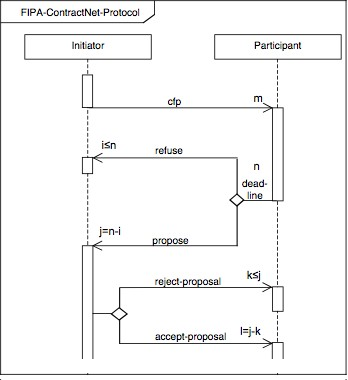
\includegraphics[scale=0.59]{fipa.png}
\end{center}

\newpage

%%%%%%%%%%%%%%%%%%%%%%%%%%
\section{Desenvolvimento}

\subsection{Plataforma/ferramenta utilizada e ambiente de desenvolvimento} 

A ferramenta escolhida para o desenvolvimento deste trabalho foi JADE. JADE é uma framework que permite o desenvolvimento de sistemas multiagente e é compatível com FIPA, isto é, segue os padrões de software estabelecidos para agentes heterogéneos e interativos e para sistemas baseados em agentes.

O projeto foi desenvolvido utilizando o IntelliJ IDEA Community Edition no sistema operativo Windows 10.

\subsection{Estrutura da aplicação} 

\begin{center}
\hspace*{-3.2cm}
	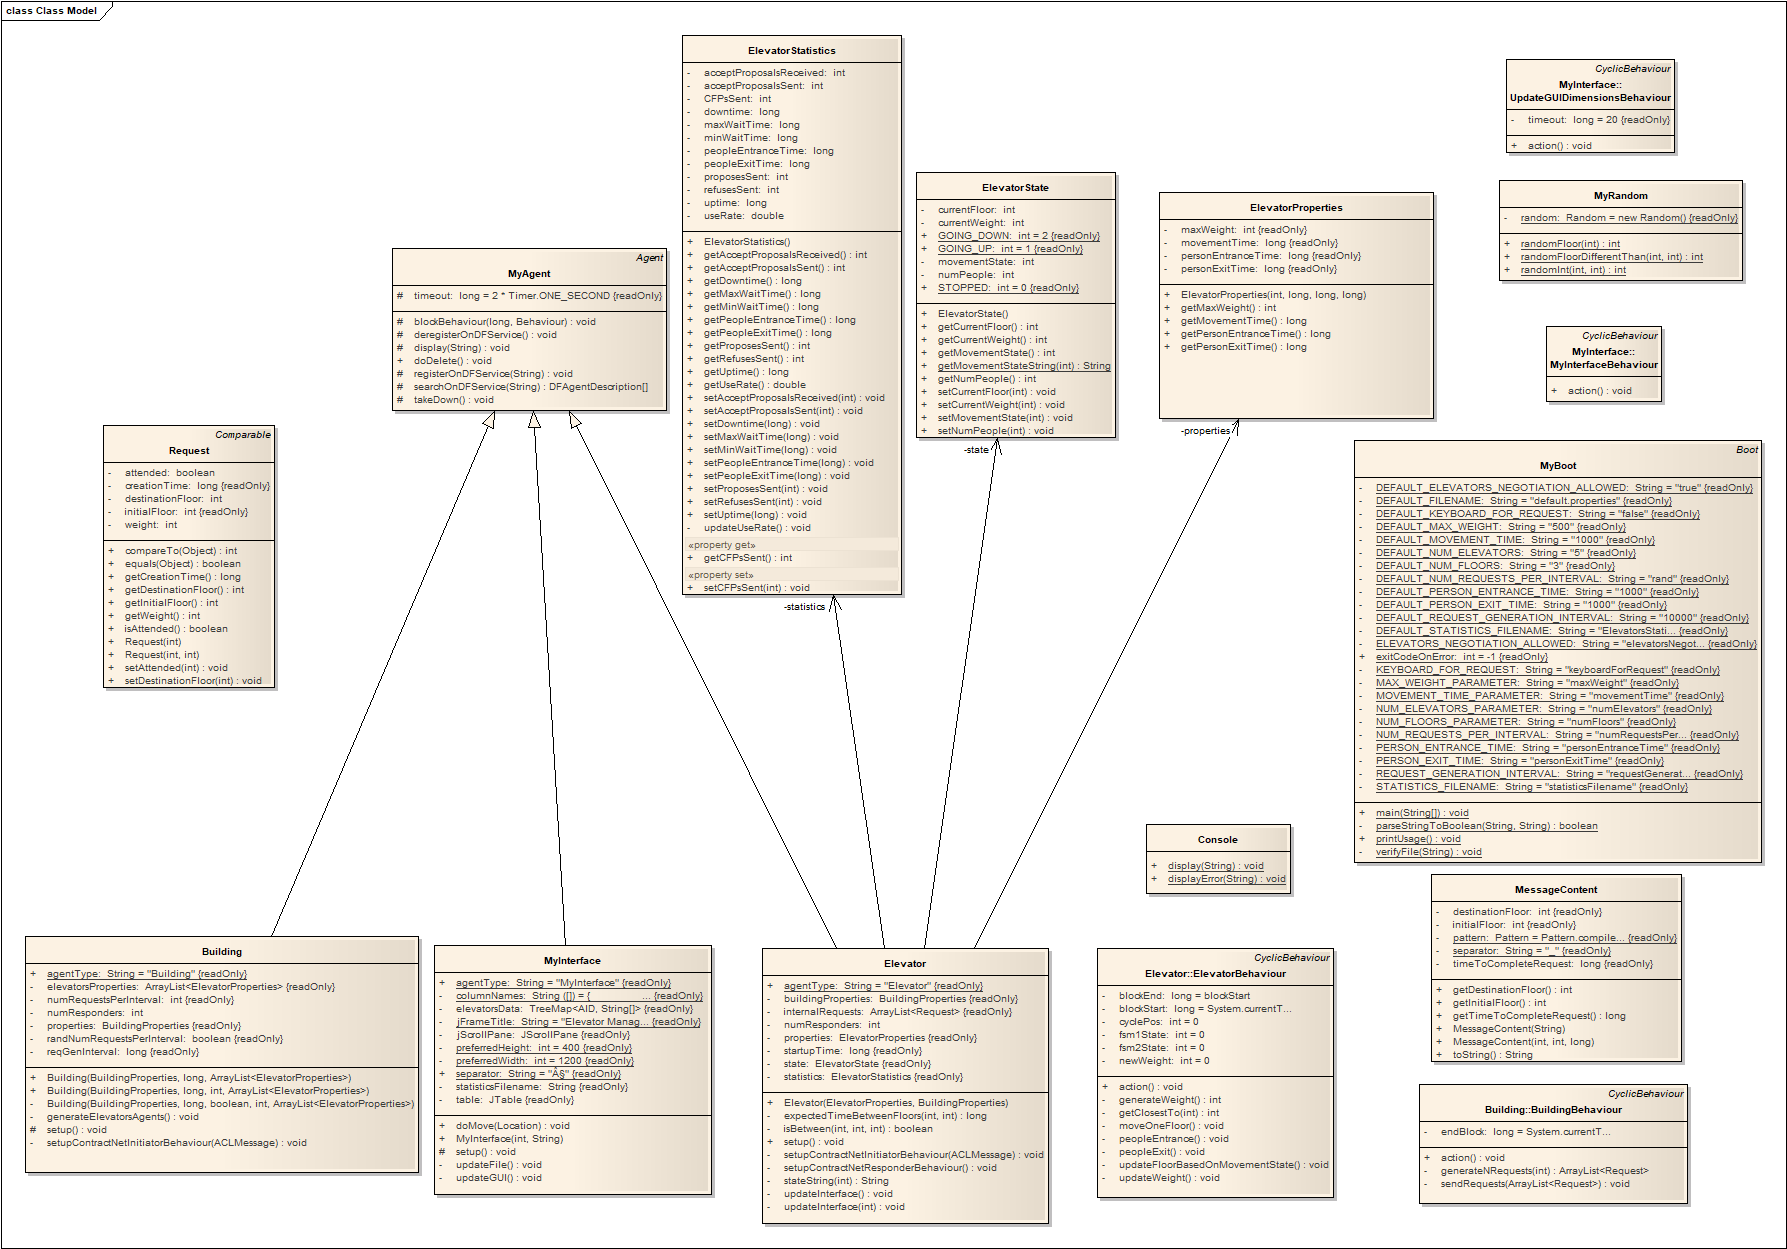
\includegraphics[scale=0.3]{class_model.png}\linebreak\linebreak
\end{center}

\subsection{Detalhes relevantes da implementação} 

\newpage

%%%%%%%%%%%%%%%%%%%%%%%%%%
\section{Experiências}

De seguida, serão detalhadas algumas das experiências efetuadas de forma a ser possível tirar conclusões dos resultados, analisando as estratégias implementadas e a sua adaptação à variação das condições. De notar que para a realização destas experiências, o tempo de movimentação dos elevadores e a capacidade máxima é igual para todos os elevadores. No entanto, o nosso programa permite que os valores sejam diferentes. Pensamos que o mais correto para conseguirmos concluir algo sobre as estratégias era que todos os elevadores tivessem as mesmas condições entre eles, fazendo-as variar (de igual forma entre eles) de experiência para experiência, pois caso contrário iriam existir elevadores a comportarem-se de uma melhor forma entre eles e não implicaria que fosse devido à estratégia.

Todos os resultados foram recolhidos após 2 minutos a correr o programa.

\subsection{Experiência 1}

\subsubsection{Condições iniciais}

\begin{itemize}
\item \textbf{numFloors}=10
\item \textbf{numElevators}=3
\item \textbf{requestGenerationInterval}=10000(ms)
\item \textbf{numRequestsPerInterval}=2
\item \textbf{maxWeigt Elevator 0,1,2}=[500, 500, 500]
\item \textbf{movementTime Elevator 0, 1, 2}=[1000, 1000, 1000]
\end{itemize}

\subsubsection{Objetivo} 

O objetivo desta experiência consiste em comparar os resultados das várias estratégias implementadas com as mesmas condições para todos os elevadores.

\subsubsection{Resultados}

Utilizando a primeira estratégia,

\begin{table}[h]
\centering
\hspace*{-3.2cm}
\begin{tabular}{@{}llllllllll@{}}
\toprule
Agent     & \begin{tabular}[c]{@{}l@{}}CFPs\\ sent \end{tabular} & \begin{tabular}[c]{@{}l@{}}Proposes\\ sent\end{tabular} & \begin{tabular}[c]{@{}l@{}}Refuses\\ sent\end{tabular} & \begin{tabular}[c]{@{}l@{}}Accept\\ proposals sent\end{tabular} & \begin{tabular}[c]{@{}l@{}}Accept proposals\\ received\end{tabular} & \begin{tabular}[c]{@{}l@{}}Max wait\\ time (ms)\end{tabular} & \begin{tabular}[c]{@{}l@{}}Uptime\\ (ms)\end{tabular} & \begin{tabular}[c]{@{}l@{}}Downtime\\ (ms)\end{tabular} &\begin{tabular}[c]{@{}l@{}}Use \\rate (\%) \end{tabular} \\ \midrule
Elevator0 & 17        & 32            & 14           & 5                                                               & 15                                                                  & 7010                                                         & 57166                                                 & 42024                                                   & 57.63         \\
Elevator1 & 10        & 30            & 22           & 4                                                               & 13                                                                  & 2022                                                         & 64086                                                 & 53114                                                   & 54.68         \\
Elevator2 & 10        & 29            & 26           & 3                                                               & 10                                                                  & 4003                                                         & 63165                                                 & 44032                                                   & 58.92         \\
Average   & 12.22     & 30.33         & 20.67        & 4                                                               & 12.67                                                               & 4345                                                         & 61472                                                 & 46390                                                   & 57.1          \\ \bottomrule
\end{tabular}
\end{table}

\newpage

Utilizando a segunda estratégia,

\begin{table}[h]
\centering
\hspace*{-3.2cm}
\begin{tabular}{@{}llllllllll@{}}
\toprule
Agent     & \begin{tabular}[c]{@{}l@{}}CFPs\\ sent \end{tabular} & \begin{tabular}[c]{@{}l@{}}Proposes\\ sent\end{tabular} & \begin{tabular}[c]{@{}l@{}}Refuses\\ sent\end{tabular} & \begin{tabular}[c]{@{}l@{}}Accept\\ proposals sent\end{tabular} & \begin{tabular}[c]{@{}l@{}}Accept proposals\\ received\end{tabular} & \begin{tabular}[c]{@{}l@{}}Max wait\\ time (ms)\end{tabular} & \begin{tabular}[c]{@{}l@{}}Uptime\\ (ms)\end{tabular} & \begin{tabular}[c]{@{}l@{}}Downtime\\ (ms)\end{tabular} &\begin{tabular}[c]{@{}l@{}}Use \\rate (\%) \end{tabular} \\ \midrule
Elevator0 & 12        & 27            & 16           & 1                                                               & 13                                                                  & 4045                                                         & 50078                                                 & 64040                                                   & 43.88         \\
Elevator1 & 10        & 31            & 15           & 3                                                               & 10                                                                  & 7413                                                         & 33428                                                 & 81782                                                   & 29.01         \\
Elevator2 & 8        & 29            & 19           & 4                                                               & 10                                                                  & 2022                                                         & 47246                                                 & 73067                                                   & 39.27         \\
Average   & 10     & 29         & 16.67        & 2.67                                                               & 11                                                               & 4493                                                         & 4354                                                 & 72963                                                   & 37.39          \\ \bottomrule
\end{tabular}
\end{table}

\subsection{Experiência 2}

\subsubsection{Condições iniciais}

\begin{itemize}
\item \textbf{numFloors}=10
\item \textbf{numElevators}=3
\item \textbf{requestGenerationInterval}=10000(ms)
\item \textbf{numRequestsPerInterval}=2
\item \textbf{maxWeigt Elevator 0,1,2}=[500, 500, 500]
\item \textbf{movementTime Elevator 0, 1, 2}=[300, 300, 300]
\end{itemize}

\subsubsection{Objetivo} 

O objetivo desta experiência consiste em comparar os resultados das várias estratégias implementadas com as mesmas condições para todos os elevadores, mas com velocidade mais rápida comparada com a experiência anterior.

\subsubsection{Resultados}

Utilizando a primeira estratégia,

\begin{table}[h]
\centering
\hspace*{-3.2cm}
\begin{tabular}{@{}llllllllll@{}}
\toprule
Agent     & \begin{tabular}[c]{@{}l@{}}CFPs\\ sent \end{tabular} & \begin{tabular}[c]{@{}l@{}}Proposes\\ sent\end{tabular} & \begin{tabular}[c]{@{}l@{}}Refuses\\ sent\end{tabular} & \begin{tabular}[c]{@{}l@{}}Accept\\ proposals sent\end{tabular} & \begin{tabular}[c]{@{}l@{}}Accept proposals\\ received\end{tabular} & \begin{tabular}[c]{@{}l@{}}Max wait\\ time (ms)\end{tabular} & \begin{tabular}[c]{@{}l@{}}Uptime\\ (ms)\end{tabular} & \begin{tabular}[c]{@{}l@{}}Downtime\\ (ms)\end{tabular} &\begin{tabular}[c]{@{}l@{}}Use \\rate (\%) \end{tabular} \\ \midrule
Elevator0 & 11        & 27            & 11           & 3                                                               & 12                                                                  & 3172                                                         & 35584                                                 & 82124                                                   & 30.23         \\
Elevator1 & 3        & 25            & 21           & 0                                                               & 5                                                                  & 1905                                                         & 8693                                                 & 28148                                                   & 23.60        \\
Elevator2 & 11        & 27            & 11           & 3                                                               & 13                                                                  & 3866                                                         & 19886                                                 & 86794                                                   & 18.64         \\
Average   & 8.33     & 26.33         & 14.33        & 2                                                               & 10                                                               & 2981                                                         & 21388                                                 & 65689                                                   & 24.16          \\ \bottomrule
\end{tabular}
\end{table}

Utilizando a segunda estratégia,

\begin{table}[h]
\centering
\hspace*{-3.2cm}
\begin{tabular}{@{}llllllllll@{}}
\toprule
Agent     & \begin{tabular}[c]{@{}l@{}}CFPs\\ sent \end{tabular} & \begin{tabular}[c]{@{}l@{}}Proposes\\ sent\end{tabular} & \begin{tabular}[c]{@{}l@{}}Refuses\\ sent\end{tabular} & \begin{tabular}[c]{@{}l@{}}Accept\\ proposals sent\end{tabular} & \begin{tabular}[c]{@{}l@{}}Accept proposals\\ received\end{tabular} & \begin{tabular}[c]{@{}l@{}}Max wait\\ time (ms)\end{tabular} & \begin{tabular}[c]{@{}l@{}}Uptime\\ (ms)\end{tabular} & \begin{tabular}[c]{@{}l@{}}Downtime\\ (ms)\end{tabular} &\begin{tabular}[c]{@{}l@{}}Use \\rate (\%) \end{tabular} \\ \midrule
Elevator0 & 3        & 24            & 10           & 1                                                               & 6                                                                  & 3808                                                         & 6924                                                 & 38217                                                   & 15.34         \\
Elevator1 & 7        & 24            & 6           & 2                                                               & 9                                                                  & 1528                                                         & 9952                                                 & 93882                                                   & 9.59         \\
Elevator2 & 5        & 25            & 7           & 1                                                               & 11                                                                  & 1576                                                         & 13751                                                 & 90953                                                   & 13.13         \\
Average   & 5     & 24.33         & 7.67        & 1.33                                                               & 8.67                                                               & 2304                                                         & 10209                                                 & 74351                                                   &  12.69         \\ \bottomrule
\end{tabular}
\end{table}

\subsection{Experiência 3}

\subsubsection{Condições iniciais}

\begin{itemize}
\item \textbf{numFloors}=5
\item \textbf{numElevators}=3
\item \textbf{requestGenerationInterval}=10000(ms)
\item \textbf{numRequestsPerInterval}=2
\item \textbf{maxWeigt Elevator 0,1,2}=[500, 500, 500]
\item \textbf{movementTime Elevator 0, 1, 2}=[1000, 1000, 1000]
\end{itemize}

\subsubsection{Objetivo} 

O objetivo desta experiência consiste em comparar os resultados das várias estratégias implementadas com as mesmas condições para todos os elevadores, mas com um número de pisos inferior.

\subsubsection{Resultados}

Utilizando a primeira estratégia,

\begin{table}[h]
\centering
\hspace*{-3.2cm}
\begin{tabular}{@{}llllllllll@{}}
\toprule
Agent     & \begin{tabular}[c]{@{}l@{}}CFPs\\ sent \end{tabular} & \begin{tabular}[c]{@{}l@{}}Proposes\\ sent\end{tabular} & \begin{tabular}[c]{@{}l@{}}Refuses\\ sent\end{tabular} & \begin{tabular}[c]{@{}l@{}}Accept\\ proposals sent\end{tabular} & \begin{tabular}[c]{@{}l@{}}Accept proposals\\ received\end{tabular} & \begin{tabular}[c]{@{}l@{}}Max wait\\ time (ms)\end{tabular} & \begin{tabular}[c]{@{}l@{}}Uptime\\ (ms)\end{tabular} & \begin{tabular}[c]{@{}l@{}}Downtime\\ (ms)\end{tabular} &\begin{tabular}[c]{@{}l@{}}Use \\rate (\%) \end{tabular} \\ \midrule
Elevator0 & 10        & 30            & 13           & 3                                                               & 11                                                                  & 2002                                                         & 27993                                                 & 91489                                                   & 23.43         \\
Elevator1 & 4        & 29            & 20           & 4                                                               & 7                                                                  & 1001                                                         & 16134                                                 & 105341                                                   & 13.3        \\
Elevator2 & 13        & 30            & 10           & 1                                                               & 16                                                                  & 3003                                                         & 37062                                                 & 74525                                                   & 33.2         \\
Average   & 9     & 29.67         & 14.33        & 2.67                                                               & 11.33                                                               & 2002                                                         & 27063                                                 & 90451                                                   & 23.31          \\ \bottomrule
\end{tabular}
\end{table}

Utilizando a segunda estratégia,

\begin{table}[h]
\centering
\hspace*{-3.2cm}
\begin{tabular}{@{}llllllllll@{}}
\toprule
Agent     & \begin{tabular}[c]{@{}l@{}}CFPs\\ sent \end{tabular} & \begin{tabular}[c]{@{}l@{}}Proposes\\ sent\end{tabular} & \begin{tabular}[c]{@{}l@{}}Refuses\\ sent\end{tabular} & \begin{tabular}[c]{@{}l@{}}Accept\\ proposals sent\end{tabular} & \begin{tabular}[c]{@{}l@{}}Accept proposals\\ received\end{tabular} & \begin{tabular}[c]{@{}l@{}}Max wait\\ time (ms)\end{tabular} & \begin{tabular}[c]{@{}l@{}}Uptime\\ (ms)\end{tabular} & \begin{tabular}[c]{@{}l@{}}Downtime\\ (ms)\end{tabular} &\begin{tabular}[c]{@{}l@{}}Use \\rate (\%) \end{tabular} \\ \midrule
Elevator0 & 3        & 26            & 19           & 1                                                               & 6                                                                  & 1001                                                         & 12013                                                 & 71402                                                   & 14.4        \\
Elevator1 & 12        & 26            & 10           & 2                                                               & 13                                                                  & 5005                                                         & 44285                                                 & 69131                                                   & 39.05         \\
Elevator2 & 9        & 26            & 13           & 2                                                               & 10                                                                  & 2003                                                         & 51739                                                 & 62678                                                   & 45.22         \\
Average   & 8     & 26         & 14        & 1.67                                                            & 9.67                                                               & 2670                                                         & 36012                                                 & 67737                                                   &  32.89         \\ \bottomrule
\end{tabular}
\end{table}

\subsection{Experiência 4}

\subsubsection{Condições iniciais}

\begin{itemize}
\item \textbf{numFloors}=20
\item \textbf{numElevators}=3
\item \textbf{requestGenerationInterval}=10000(ms)
\item \textbf{numRequestsPerInterval}=5
\item \textbf{maxWeigt Elevator 0,1,2}=[500, 500, 500]
\item \textbf{movementTime Elevator 0, 1, 2}=[1000, 1000, 1000]
\end{itemize}

\subsubsection{Objetivo} 

O objetivo desta experiência consiste em comparar os resultados das várias estratégias implementadas com as mesmas condições para todos os elevadores, mas com um maior número de pedidos por intervalo e um maior número de pisos.

\subsubsection{Resultados}

Utilizando a primeira estratégia,

\begin{table}[h]
\centering
\hspace*{-3.2cm}
\begin{tabular}{@{}llllllllll@{}}
\toprule
Agent     & \begin{tabular}[c]{@{}l@{}}CFPs\\ sent \end{tabular} & \begin{tabular}[c]{@{}l@{}}Proposes\\ sent\end{tabular} & \begin{tabular}[c]{@{}l@{}}Refuses\\ sent\end{tabular} & \begin{tabular}[c]{@{}l@{}}Accept\\ proposals sent\end{tabular} & \begin{tabular}[c]{@{}l@{}}Accept proposals\\ received\end{tabular} & \begin{tabular}[c]{@{}l@{}}Max wait\\ time (ms)\end{tabular} & \begin{tabular}[c]{@{}l@{}}Uptime\\ (ms)\end{tabular} & \begin{tabular}[c]{@{}l@{}}Downtime\\ (ms)\end{tabular} &\begin{tabular}[c]{@{}l@{}}Use \\rate (\%) \end{tabular} \\ \midrule
Elevator0 & 34        & 72            & 67           & 4                                                               & 24                                                                  & 6039                                                         & 88099                                                 & 34081                                                   & 72.11         \\
Elevator1 & 34        & 76            & 63           & 8                                                               & 33                                                                  & 14051                                                         & 79066                                                 & 42088                                                   & 65.3        \\
Elevator2 & 40        & 70            & 63           & 9                                                               & 29                                                                  & 8049                                                         & 86094                                                 & 34074                                                   & 71.65         \\
Average   & 36     & 72.67         & 64.33        & 7                                                               & 28.67                                                               & 9380                                                         & 84420                                                 & 36478                                                   & 69.69          \\ \bottomrule
\end{tabular}
\end{table}

Utilizando a segunda estratégia,

\begin{table}[h]
\centering
\hspace*{-3.2cm}
\begin{tabular}{@{}llllllllll@{}}
\toprule
Agent     & \begin{tabular}[c]{@{}l@{}}CFPs\\ sent \end{tabular} & \begin{tabular}[c]{@{}l@{}}Proposes\\ sent\end{tabular} & \begin{tabular}[c]{@{}l@{}}Refuses\\ sent\end{tabular} & \begin{tabular}[c]{@{}l@{}}Accept\\ proposals sent\end{tabular} & \begin{tabular}[c]{@{}l@{}}Accept proposals\\ received\end{tabular} & \begin{tabular}[c]{@{}l@{}}Max wait\\ time (ms)\end{tabular} & \begin{tabular}[c]{@{}l@{}}Uptime\\ (ms)\end{tabular} & \begin{tabular}[c]{@{}l@{}}Downtime\\ (ms)\end{tabular} &\begin{tabular}[c]{@{}l@{}}Use \\rate (\%) \end{tabular} \\ \midrule
Elevator0 & 33        & 72            & 52           & 7                                                               & 27                                                                  & 19054                                                         & 77101                                                 & 43965                                                   & 63.69        \\
Elevator1 & 32        & 73            & 52           & 7                                                               & 28                                                                  & 14059                                                         & 90101                                                 & 31088                                                   & 74.35         \\
Elevator2 & 27        & 73            & 57           & 5                                                               & 29                                                                  & 13083                                                         & 68083                                                 & 52065                                                   & 56.67         \\
Average   & 30.67     & 72.67         & 53.67        & 6.33                                                            & 28                                                               & 15399                                                         & 78428                                                 & 42373                                                   &  64.9         \\ \bottomrule
\end{tabular}
\end{table}

\newpage

%%%%%%%%%%%%%%%%%%%%%%%%%%
\section{Conclusões}

\subsection{Da análise dos resultados das experiências levadas a cabo} 

\subsection{Do desenvolvimento do trabalho e aplicabilidade de SMA ao cenário proposto}

\newpage

%%%%%%%%%%%%%%%%%%%%%%%%%%
\section{Melhoramentos}

\subsection{Sugestões para melhoramentos a introduzir no programa}

De forma a conseguirmos ter uma melhor comparação era importante adicionar mais estratégias de respostas aos pedidos, conseguindo assim realizar mais experiências e extraindo novas conclusões.

Achamos que a interface podia ser ligeiramente melhorada, de forma a demonstrar melhor o funcionamento dos elevadores, como eles subirem/descerem e abrirem/fechar as portas à entrada/saída dos utentes. No entanto, consideramos que as estatísticas demonstradas conseguem transmitir uma boa ideia daquilo que se está a suceder.

\newpage

%%%%%%%%%%%%%%%%%%%%%%%%%%

\section{Recursos}

\subsection{Bibliografia} 

Slides do Moodle sobre JADE

Documentação do JADE

Código fonte do JADE

\subsection{Software} 

JADE (http://jade.tilab.com/)

Eclipse IDE for Java

IntelliJ IDEA Community Edition

\subsection{Elementos do grupo}

O grupo trabalhou de forma equitativa durante as aulas práticas e houve boa comunicação entre os membros, de forma a que cada elemento soubesse o que estava a ser feito.

%%%%%%%%%%%%%%%%%%%%%%%%%%
\section{Apêndice}

\subsection{Manual do utilizador} 

Para conseguir correr o projeto, deve:

1. Importar o projeto;

2. Adicionar a \textit{library} do \textit{JADE} ao \textit{build path};

3. Editar o ficheiro default.properties consoante o que deseja visualizar na interface;

4. Correr, utilizando a classe MyBoot como \textit{main}.

\newpage

%%%%%%%%%%%%%%%%%%%%%%%%%%

\end{document}
